%! suppress = MissingLabel

В этой главе собраны некоторые общие знания о типах.
Также, мы получим различные эквивалентные представления рекурсивных типов данных (иначе говоря, коллекций).
Многие концепции являются частными случаями этого многообразия.

Разделы~\ref{subsec:variance}, ~\ref{subsec:isomorphism} в основном следуют~\cite[глава 1]{maguire-types}.

\subsection{Вариантность} \label{subsec:variance}

В этом параграфе мы будем рассматривать тему с точки зрения программирования~\cite[глава 3]{maguire-types}, не отдавая должного теории категорий.
Восполнить пробел можно с помощью замечательной статьи, написанной в жанре пьесы~\cite{hinze2012functional}.

\vocab{Ковариантный функтор} --- пара из некоторого типового конструктора \texttt{F} и операции на функциях \texttt{fmap :: (a -> b) -> (F a -> F b)}.
Плюс законы о том, что \texttt{fmap} уважает \texttt{id} и композицию.

\begin{minted}{haskell}
    class Functor f where
      fmap :: (a -> b) -> (f a -> f b)
\end{minted}

\begin{figure}[H]
    \centering
    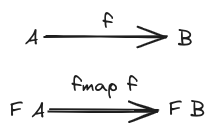
\includegraphics[width=0.3\textwidth]{figs/functor}
\end{figure}

\vocab{Контравариантный функтор} --- пара из типового конструктора и операции на функциях, разворачивающей стрелку.
Плюс соответствующие законы.

\begin{minted}{haskell}
    class Contravariant f where
      contramap :: (a -> b) -> (f b -> f a)
\end{minted}

\begin{figure}[H]
    \centering
    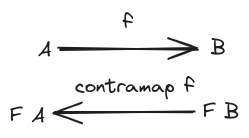
\includegraphics[width=0.3\textwidth]{figs/contra-functor}
\end{figure}

Типовой конструктор можно объявить ковариантным или контравариантным функтором (или никаким из них) относительно некоторого типового параметра в зависимости от вида декларации соответствующих конструкторов данных.
А именно, от знака позиций, в которых входит этот типовой параметр в тип.

Разовьём интуитивное понимание знаков позиций.
Тип \mintinline{haskell}{A} входит в положительной позиции в \mintinline{haskell}{B} если его значение можно извлечь из \mintinline{haskell}{B}.
И наоборот, тип \mintinline{haskell}{A} входит в отрицательной позиции, если его значение нужно, наоборот, предоставить.
Рассмотрим знаки позиций типов в базовых типовых конструкторах:
\begin{center}
    \begin{tabular}[h]{|c|c|c|}
        \hline
        Тип                              & знак позиции \mintinline{haskell}{A} & знак позиции \mintinline{haskell}{B} \\
        \hline
        \mintinline{haskell}{Either A B} & $+$                                  & $+$                                  \\
        \mintinline{haskell}{(A, B)}     & $+$                                  & $+$                                  \\
        \mintinline{haskell}{A -> B}     & $-$                                  & $+$                                  \\
        \hline
    \end{tabular}
\end{center}

Действительно, из суммы и произведения можно извлечь компоненты с помощью паттерн-матчинга, а из стрелки можно получить правый тип апплицируя её к аргументу.
В то же время значение типа слева от стрелки нужно предоставить.

На плюс и минус действуют интуитивные алгебраические законы при рассмотрении более сложных типов.
Рассмотрим на примере \mintinline{haskell}{f :: ((A, B) -> C) -> (D, E)}.
\begin{itemize}
    \item Плюс на плюс даёт плюс.
    Действительно, нужно лишь применить две элиминации вместо одной, чтобы получить заветный тип.
    В нашем примере, чтобы получить \mintinline{haskell}{D}, нужно сначала апплицировать функцию, а потом разобрать пару.
    \item Плюс на минус (и наоборот) даёт минус.
    Действительно, \mintinline{haskell}{C} нам нужно предоставить: \mintinline{haskell}{f (\ab -> provideC)}.
    \item Минус на минус даёт плюс.
    Пару \mintinline{haskell}{(A, B)} нам предоставляют: \mintinline{haskell}{f (\ab -> ...)}.
\end{itemize}

\begin{task}
    Убедитесь что плюс на минус даёт минус.
\end{task}

Возвращаясь к функторам, если типовой параметр входит в декларацию только в положительных позициях, типовой конструктор можно объявить ковариантным функтором относительно этого параметра.
Если в только в отрицательных~--- контравариантным функтором.
Если в обоих, то никаким функтором объявить нельзя.
Соответственно, будем называть типовые параметры ковариантными, контравариантными и инвариантными.

\begin{task}
    Объявите \mintinline{haskell}{instance Contravariant F} для \mintinline{haskell}{data F a = L (a -> ()) | R Int}.
\end{task}

Таким образом, можно понимать ковариантный функтор как вычисление, результат которого можно пост-обработать, а контравариантный функтор --- как вычисление, аргументы которого можно пред-обработать.

Тип от двух положительных параметров можно объявить \vocab{бифунктором}:
\begin{minted}{haskell}
    class Bifunctor f where
      bimap :: (a -> c) -> (b -> d) -> f a b -> f c d
\end{minted}

Тип от двух параметров, положительного и отрицательного, --- \vocab{профунктором}:
\begin{minted}{haskell}
    class Profunctor p where
      dimap :: (c -> a) -> (b -> d) -> p a b -> p c d
\end{minted}

Профункторы являются некоторыми обобщениями функциональной стрелки.
Например, если у нас есть SQL запрос, который по данным возвращает результат, его можно объявить профунктором с семантикой --- добавить пред-обработку входных данных и пост-обработку выходных:
\begin{minted}{haskell}
    dimap serialize deserialize (query :: Sql Text Text) :: Sql Age [User]
\end{minted}

Также понятие вариантности часто встречается в объектно ориентированных языках (да и вообще в теории подтипизации) для обозначения возможности дополнить отношение подтипизации на полиморфные типы.

Действительно, \vocab{отношение подтипизации} \texttt{B <: A} говорит о том, что значение типа \texttt{B} безопасно использовать в позиции, где ожидается значение типа \texttt{A}.
Иначе говоря, существует функция \texttt{upcast :: B -> A}.
Если типовой конструктор \texttt{F a} ковариантен относительно параметра \texttt{a}, то по \texttt{upcast} найдётся \texttt{upcast' :: F B -> F A}.
То есть отношение подтипизации также автоматически включает \texttt{F B <: F A}.
Контравариантный случай аналогично.

\begin{task}
    Убедитесь в вашем любимом языке с подтипизацией и поддержкой вариантности, что минус на минус даёт плюс.
\end{task}

\subsection{Изоморфизм} \label{subsec:isomorphism}

Пусть нам нужно спроектировать функцию или модель данных.
Мы начинаем с декларации типа, как её выбрать и из каких вариантов?
Для начала поймём, когда два типа взаимозаменимы, для этого рассмотрим понятия изоморфизма.

Два типа \texttt{A} и \texttt{B} называются \vocab{изоморфными} (обозначают \texttt{A $\iso$ B}) тогда и только тогда, когда существует такая пара функций \texttt{to :: A -> B} и \texttt{from :: B -> A}, что\footnote{Под равенством термов можно понимать разное, например, $\alpha\beta\gamma$-эквивалентность. Мы будем пользоваться \vocab{экстенсиональным равенством} для функций~--- две функции равны, когда равны их результаты на всех входах. \url{https://ncatlab.org/nlab/show/function+extensionality}}
\begin{minted}{c}
    to . from = id
    from . to = id
\end{minted}

Иначе говоря, между обитателями таких типов можно установить взаимно-однозначное соответствие.
Легко понять, что со смысловой точки зрения не принципиально, какой из изоморфных типов использовать --- их можно заменять друг на друга, добавляя вызовы функций перехода.
Такие два типа заключают в себе одинаковое ``количество информации''.
Например, типы \mintinline{haskell}|Bool| и \mintinline{haskell}|Maybe ()| в этом смысле совершенно взаимозаменимы.
Покажем это, предъявив пару взаимообратных функций\footnote{Нужно не забыть показать взаимообратность функций, но это делается тривиально перебором входов (может быть с помощью индукции) и редукцией.}:
\begin{minted}{haskell}
    to :: Bool -> Maybe ()
    to b = if b then Just () else Nothing

    from :: Maybe () -> Bool
    from m = case m of Nothing -> False; Just () -> True
\end{minted}

Несмотря на смысловую взаимозаменимость, для кодирования информации о том, передал ли пользователь программе определённый флаг, мы, скорее всего, воспользуемся типом \mintinline{haskell}|Bool| ввиду нефункциональных соображений о читабельности кода.
Аналогично можно рассматривать соображения эффективности.

С категорным взглядом на происходящее можно ознакомиться в~\cite{hinze2010reason}.
Мы же придерживаемся теоретико-множественной интерпретации типов.

\subsubsection{Кардинальность: суммы, произведения, экспоненты} \label{subsubsec:cardinality}

Типы можно воспринимать как синтаксис для записи множеств, а населяющие их термы~--- как синтаксические записи элементов этих множеств.
Так терм \mintinline{haskell}|(True, False)|~--- запись элемента множества пар, записываемого в синтаксисе типов как \mintinline{haskell}|(Bool, Bool)| (вместо математического $\mathbb{B}\times\mathbb{B}$).
Или же терм \mintinline{haskell}|\x -> x + 1| является записью функции прибавляющей единицу из множества функций над целыми числами, записываемого как \mintinline{haskell}|Integer -> Integer| (вместо математического $\mathbb{Z}\to\mathbb{Z}$).

Заметим, что два типа изоморфны, если соответствующие им множества имеют одинаковое количество элементов.
Более того, таких изоморфизмов $n!$ в случае конечности множеств.
Научимся определять количество таких элементов.
С помощью $|\cdot|$ будем записывать \vocab{кардинальность} типа~--- количество элементов в соответствующем множестве.

\begin{center}
    \begin{tabular}{|l|c|}
        \hline
        Тип и его декларация                                                                                                                                                                            & кардинальность \\
        \hline
        \mintinline{haskell}{data Void}                                                                                                                                                                 & $0$            \\
        \mintinline{haskell}{data Unit = Unit}\footnote{\mintinline{haskell}|Unit| записывается в Haskell с помощью специального синтаксиса \mintinline{haskell}|()|, означающем как бы пустой кортеж.} & $1$ \\
        \mintinline{haskell}{data Bool = False | True}                                                                                                                                                  & $2$            \\
        \hline
    \end{tabular}
\end{center}

Идея алгебраических типов данных в том, что сложные типы можно строить из простых с помощью операции $+$ (``или'') и операции $\times$ (``и'')\footnote{\url{https://stanford-cs242.github.io/f18/lectures/02-2-algebraic-data-types.html}}:
\begin{center}
    \begin{tabular}{|l|c|}
        \hline
        Тип                                                      & кардинальность   \\
        \hline
        \mintinline{haskell}{data Either a b = Left a | Right b} & $|a| + |b|$      \\
        \mintinline{haskell}{data Pair a b = Pair a b}           & $|a| \times |b|$ \\
        \hline
    \end{tabular}
\end{center}

Посчитаем количество обитателей различных типов (вы можете убедиться в справедливости заключения перебрав все термы вручную):
\begin{itemize}
    \item \mintinline{haskell}{|Either Unit (Eigher Bool Bool)| = |Unit| + (|Bool| + |Bool|) = 5}.
    \item \mintinline{haskell}{Pair (Either Bool Unit) (Pair Unit Void)| = 0} ~--- тип \mintinline{haskell}|Void| не населён, как и кортеж, его включающий.
    \item Если \mintinline{haskell}{data Example = FirstAlternative Bool | AnotherOne Unit Bool Bool}, то \\\mintinline{haskell}{|Example| = |Bool| + |Unit| * |Bool| * |Bool| = 2 + 1 * 2 * 2 = 6}.
\end{itemize}

Функциональную стрелку называют экспоненциальным типом.
Действительно, комбинаторно количество обитателей \mintinline{haskell}|A -> B| вычисляется как \[|A \to B| = |B|^{|A|}\]

Так как проектировать типы?
Тому есть несколько соображений:
\begin{itemize}
    \item В типе должно быть не меньше элементов, чем в предметной области, все необходимые объекты были представимы.
    \item В типе должно быть как можно меньше элементов, которых нет в предметной области, чтобы пространство ошибок было минимальным.
    \item Далее среди изоморфных типов выбирается оптимальный исходя из нефункциональных требований.
\end{itemize}

Прежде чем работать с некоторым объектом предметной области, информацию о нём, в соответствии со вторым правилом, следует привести в максимально структурное представление, дающее наибольшее количество гарантий\footnote{\url{https://lexi-lambda.github.io/blog/2019/11/05/parse-don-t-validate/}}.

\subsubsection{Алгебраическое представление типа} \label{subsubsec:type-algebra}

Как мы увидели выше, чтобы показать наличие изоморфизма между двумя типами можно либо предъявить пару взаимообратных функций, либо показать, что кардинальности этих двух типов совпадают.
В этом разделе мы научимся сопоставлять типу некоторую алгебраическую запись, отражающую его структуру и кардинальность.
Так, мы сможем синтаксическими преобразованиями формул получать эквивалентные записи, из которых будем восстанавливать типы, заведомо изоморфные данному\footnote{\url{https://codewords.recurse.com/issues/three/algebra-and-calculus-of-algebraic-data-types}}.

В основу алгебраического представления положим вычисление кардинальности типов.
Фактически мы забываем несущественную для изоморфизма информацию об именах конструкторов данных и конструкторов типов, то есть переходим к структурной типизации.
\begin{center}
    \begin{tabular}{|p{0.5\textwidth}|c|}
        \hline
        Тип                                                      & алгебраическая формула      \\
        \hline
        \mintinline{haskell}{data Void}                          & $0$                         \\
        \mintinline{haskell}{data Unit = Unit}                   & $1$                         \\
        \mintinline{haskell}{data Bool = False | True}           & $1 + 1$ (обозначим как $2$) \\
        \mintinline{haskell}{data Maybe a = Nothing | Just a}    & $1 + a$                     \\
        \mintinline{haskell}{data Either a b = Left a | Right b} & $a + b$                     \\
        \mintinline{haskell}{data Pair a b = Pair a b}           & $a \times b$                \\
        \mintinline{haskell}{a -> b}                             & $b^a$                       \\
        \hline
    \end{tabular}
\end{center}

\begin{task}
    Запишите в алгебраическом виде следующий тип:
    \begin{minted}{haskell}
        data T a b = Undefined | Defined a (a -> b)
    \end{minted}
\end{task}

В качестве отношения эквивалентности, будем использовать изоморфизм соответствующих типов.
В такой интерпретации, классические свойства алгебраических операций сохраняются (рис.~\ref{fig:school-alg}).
Действительно, например:
\begin{minted}{haskell}
    -- ?$(c^b)^a \iso c^{a\times b}$?
    to :: (a -> b -> c) -> (a, b) -> c
    to = uncurry
    from :: ((a, b) -> c) -> a -> b -> c
    from = curry
\end{minted}

\begin{figure}
    \centering
    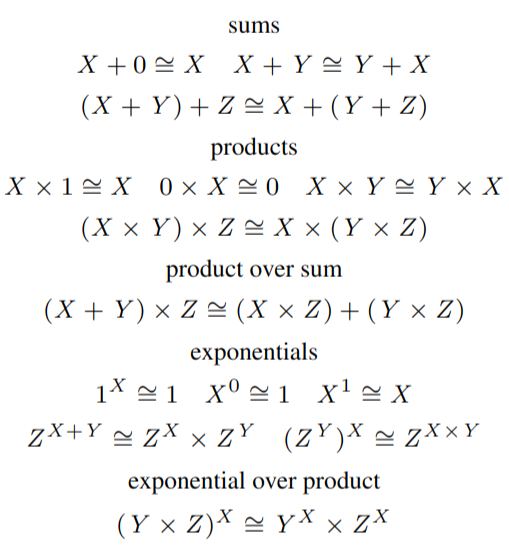
\includegraphics[width=0.4\textwidth]{figs/school-alg}
    \caption{Законы школьной алгебры ностальгии ради~\cite{hinze2010reason}.}
    \label{fig:school-alg}
\end{figure}

\begin{task}
    Покажите, что $(a + b) + c \iso a + (b + c)$.
\end{task}

\begin{task}
    Покажите, что $c^{a + b} \iso c^a\times c^b$.
\end{task}

Интересным наблюдением может быть то, что функции можно использовать как структуры данных, в соответствие с изоморфизмом $c^{a + b} \iso c^a\times c^b$.
Действительно, в таком случае аргумент функции выступает индексом (его кардинальность должна совпадать с размером коллекции).
\begin{minted}{haskell}
    -- ?$a \times a \iso a^2$?
    get :: (a, a) -> (Bool -> a)
    get (x, y) idx = if idx then x else y
    tabulate :: (Bool -> a) -> (a, a)
    tabulate f = (f True, f False)
\end{minted}

\vocab{Каноническим предствлением типа (canonical representaion)} называют сумму произведений типов:
\[
    \sum_{i}\prod_{j} t_{ij}
\]
Каноническое представление является своего рода нормальной формой, в которой можно записывать алгебраические типы (любой алгебраический тип можно по правилам привести к ней).
Легко узнать в нём вид \mintinline{haskell}{data} деклараций в Haskell.

Удивительно, но даже производная алгебраического типа имеет вполне понятную семантику.
Это контекст зиппера (zipper), структуры данных наподобие итератора, позволяющей навигироваться по структуре данных произвольной формы~\cite{huet1997zipper, mcbride2001derivative, abbott2003derivatives}.

\subsection{Рекурсивные типы} \label{subsec:recursive-types}

Рекурсивные типы, наподобие рекурсивным термам, могут включать себя в своих определениях.
Иначе говоря, рекурсивный тип изоморфен какому-то другому типу, в который он сам входит как подтип.
\begin{minted}{haskell}
    fac n = if n <= 1 then 1 else n * ?\framebox{fac}? (n - 1)
    data Nat = Zero | Suc ?\framebox{Nat}?
\end{minted}

Мы в основном посмотрим на рекурсивные типы с практической точки зрения.
Однако, их формальное теоретико-типовое описание, теоретико-категорная и теоретико-множественная интерпретации представляют отдельный интерес~\cite[часть 4]{pierce2002types}.

\subsubsection{Просто список}

Рассмотрим классический функциональный список.
Список это либо коллекция из нуля элементов, либо одного, либо двух\ldots
Алгебраически это запишется следующим образом:
\[
    L = 1 + a + a^2 + a^3 + \ldots
\]
Фактически получили тип с бесконечной записью.
Поработаем с ним как с формальным рядом.
Вынесем $a$ за скобки:
\[
    L = 1 + a \times (1 + a + a^2 + \ldots)
\]
Заметим, что выражение в скобках представляет собой список, получим такое рекурсивное уравнение\footnote{Либо можно получить то же самое, заметив, что мы имеем дело с рядом Тейлора \url{https://codewords.recurse.com/issues/three/algebra-and-calculus-of-algebraic-data-types}.}:
\[
    L = 1 + a \times L
\]
Легко видеть, что это на самом деле знакомое нам определение списка из Haskell:
\begin{minted}{haskell}
    data List a = Nil | Cons a (List a)
\end{minted}

Получим конечное нерекурсивное представление типа $L$.
Фактически, нам нужно получить тип изоморфный типу, включающему в себя исходный:
\[
    L \iso 1 + a \times L
\]
Расширим язык типов абстракцией (полиморфизмом) и решим полученное рекурсивное уравнение в стиле $\lambda$-исчисления, с помощью некоторого комбинатора неподвижной точки:
\[
    L = FIX\ap\lambda r\ldotp 1 + a \times r
\]
Закодируем это на Haskell.
В качестве комбинатора рекурсии возьмём \mintinline{haskell}{data FixList a}:
\begin{minted}{haskell}
    data ListShape a r = Either () (a, r) -- ?$\lambda a~r\ldotp 1 + a\times r$?
    data FixList a = FixList (ListShape a (FixList a))
    -- FixList a ?$\iso$? ListShape a (FixList a)
\end{minted}

Таким образом, мы разделили определение списка на две части: одна отвечает за форму типа, другая --- за рекурсию.
Иначе говоря, вместо того, чтобы сослаться на себя, тип абстрагируется по рекурсивной ссылке, которую ему предоставят снаружи.
Эта техника называется \vocab{открытой рекурсией}.
Так, пользователь может контролировать, рекурсию, чем мы в дальнейшем будем пользоваться.
Форму можно переиспользовать, например, в определении свёртки:
\begin{minted}{haskell}
    foldr :: (Either () (a, r) -> r) -> FixList a -> r
    foldr phi (FixList shape) = case shape of
      Left () -> phi (Left ())
      Right (x, xs) -> phi (Right (x, foldr phi xs))
    -- сравните с классическим определением
    foldr :: r -> (a -> r -> r) -> [a] -> r
\end{minted}

\subsubsection{Неподвижная точка функтора} \label{subsubsec:functor-fixpoint}

Абстрагируем \mintinline{haskell}{FixList} по типу-форме:
\begin{minted}{haskell}
    newtype Fix :: (Type -> Type) -> Type
    newtype Fix f = In { out :: f (Fix f) }

    data ListF a r = FNil | FCons a r
    type List a = Fix (ListF a)
\end{minted}

\begin{task}
    Какие типы будут у \mintinline{haskell}|In| и \mintinline{haskell}|out|?
\end{task}

Можно показать, что \mintinline{haskell}{[a] ?$\iso$? List a}:
\begin{minted}{haskell}
    to :: [a] -> List a
    to = \case
      [] -> In FNil
      x:xs -> In $ FCons x (to xs)

    from :: List a -> [a]
    from (In shape) = case shape of
      FNil -> []
      FCons x xs -> x : from xs
\end{minted}

Тип формы можно сделать функтором по последнему параметру.
Это позволит нам в дальнейшем заменять вхождения поддеревьев на что-то полезное.
\begin{minted}{haskell}
    instance Functor (ListF a) where
      fmap :: (rec -> other) -> ListF a rec -> ListF a other
      fmap f = \case
        FNil -> FNil
        FCons x xs -> FCons x (f xs)
\end{minted}

Таким образом, мы научились кодировать рекурсивный тип в стиле теории категорий, как неподвижную точку функтора.

\begin{task}
    Выразите следующее дерево как неподвижную точку функтора.
    Объявите инстанс функтора для типа-формы.
    \begin{minted}{haskell}
        data Tree a = Leaf a | Node a (Tree a) (Tree a)
    \end{minted}
\end{task}

\subsubsection{Схемы рекурсии} \label{subsubsec:recursion-schemas}

Подобно тому, как структурное императивное программирование, в сравнении с беспорядочным использованием \texttt{goto}, помогает рассуждать о программах, так \vocab{схемы рекурсии} позволяют алгебраически описывать свойства рекурсивных функций, в отличие от ``неструктурной'' рекурсии\footnote{\url{https://reasonablypolymorphic.com/blog/recursion-schemes/index.html}}~\cite{meijer1991functional, meijer1995bananas}.

Глобальная идея состояла в том, чтобы формулировать требуемые свойства и вычислять нужные программы подобно тому, как математики находят решения дифференциальных уравнений.
Однако, эта идея не нашла нужного развития и применения (однако, владеть алгебраическим подходом в целом полезно~\cite{maguire-algebra}).
Тем не менее это знание, с одной стороны, даёт более глубокое понимание рекурсии, с другой, пригодится нам для рассмотрения и решения главной проблемы этого курса~--- expression problem.

Для начала рассмотрим обобщённую свёртку.
Свёртка в общем смысле позволяет заменить все каждый конструктор данных в дереве на некоторую функцию.
В результате получается вычисление, имеющее доступ ко всему содержимому структуры данных, возвращающее некоторый результат агрегации:
\begin{center}
    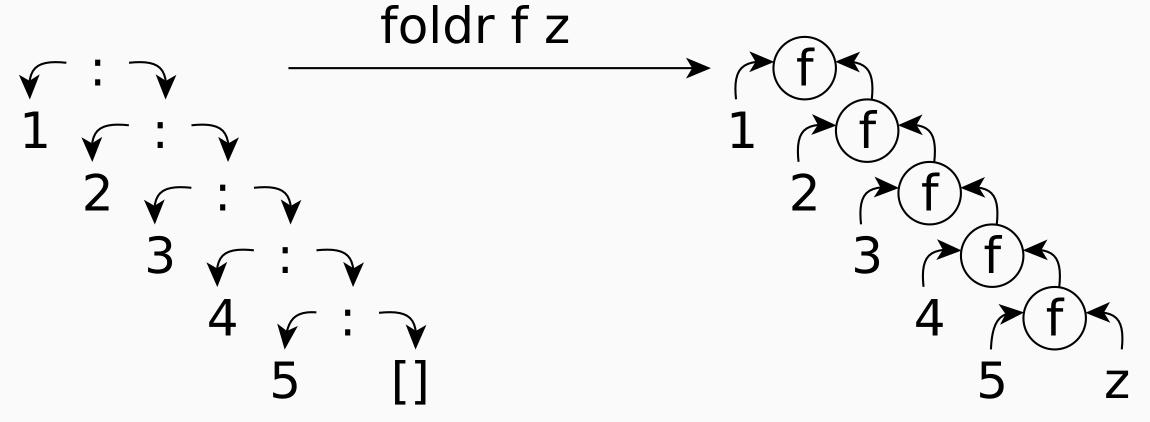
\includegraphics[width=0.5\textwidth]{figs/foldr}
\end{center}

Однако как написать свёртку, работающую для произвольного типа данных?
Функция \texttt{foldr} явно полагается на знание о конструкторах списка --- она принимает ноль-арную функцию \texttt{z} для замены \texttt{[]} и бинарную для \texttt{(:)}.
Нам поможет разделение рекурсивного типа на функтор формы и рекурсивный тип.

Универсальная свёртка называется \vocab{катаморфизмом}.
Катаморфизм сначала рекурсивно сворачивает поддеревья, добираясь к ним с помощью \mintinline{haskell}|fmap|, и оставляет результаты свёртки типа \texttt{a} вместо бывших вхождений поддеревьев.
Получается значение типа \texttt{f a}, где \texttt{f} --- какой-то функтор формы.
Далее применяется функция типа \texttt{f a -> a}, которая определяет, как свернуть один слой рекурсивной структуры, когда поддеревья уже свёрнуты.
\begin{minted}{haskell}
    cata :: Functor f => (f a -> a) -> Fix f -> a
    cata phi = phi . fmap (cata phi) . out
\end{minted}

\begin{figure}[h]
    \centering
    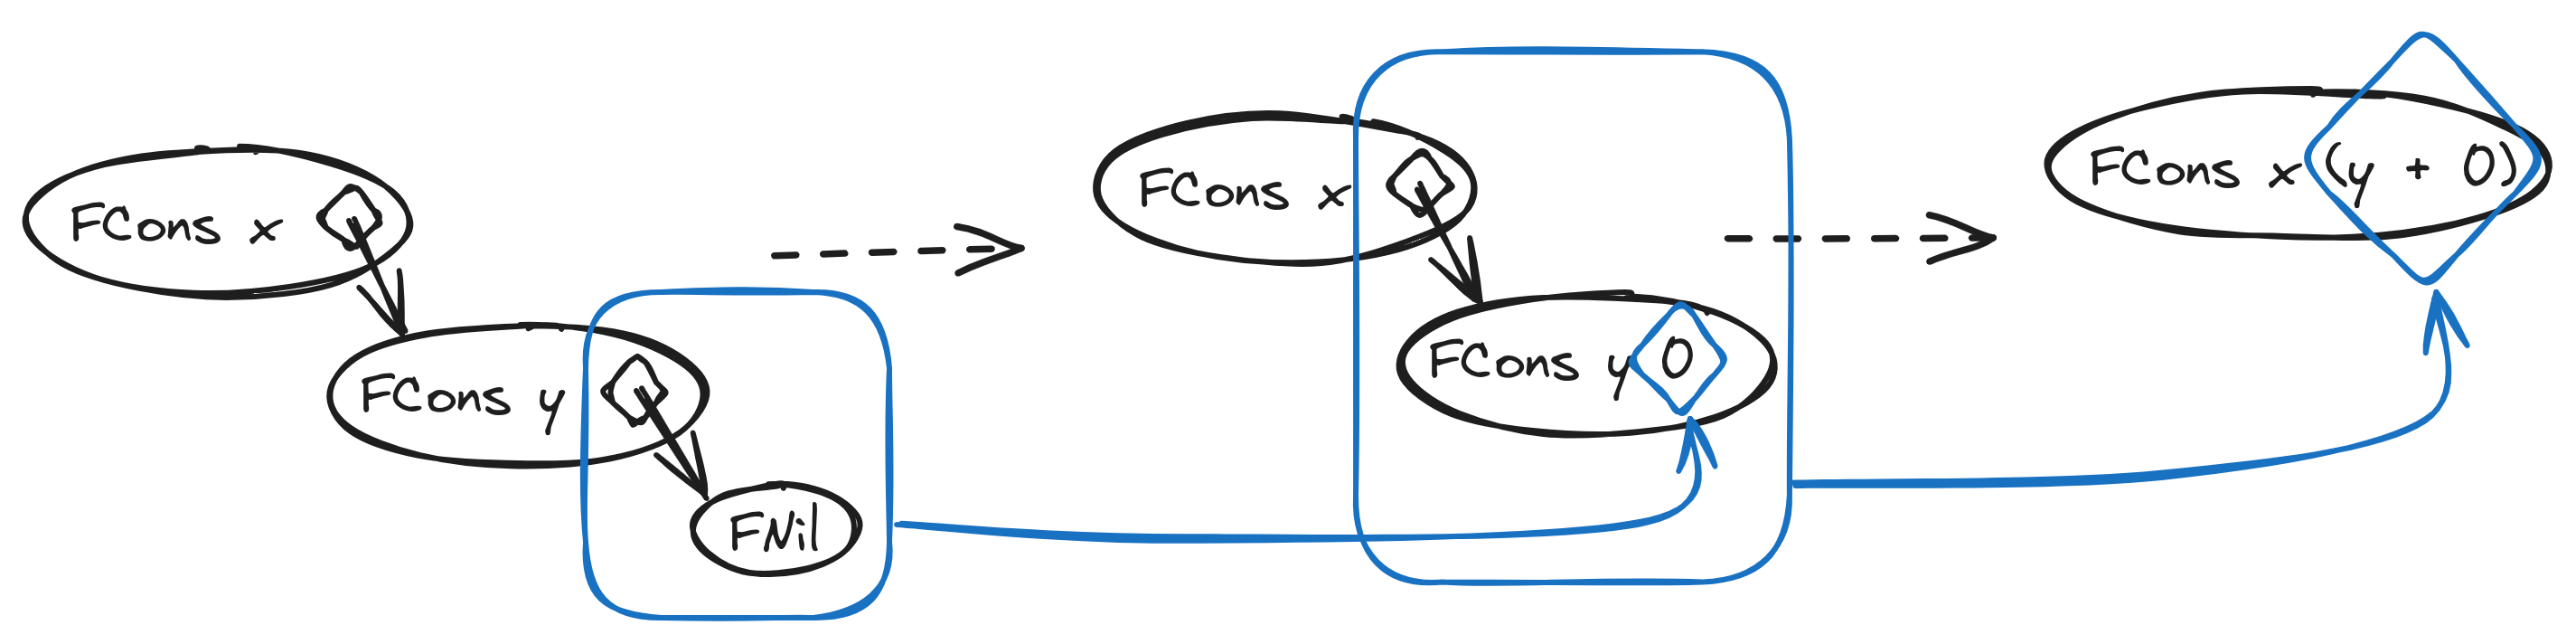
\includegraphics[width=0.8\textwidth]{figs/cataStep.excalidraw}
\end{figure}

Например, сумма списка будет выглядеть следующим образом:
\begin{minted}{haskell}
    sum :: List Int -> Int
    sum = cata \case
      FNil -> 0
      FCons x result -> x + result
\end{minted}

Функцию \texttt{f a -> a} называют \vocab{f-алгеброй}.
Действительно, если в качестве функтора \texttt{f} взять сигнатуру алгебры, а в качестве \texttt{a} носитель, то f-алгебра будет задавать некоторую интерпретацию сигнатуры:
\begin{minted}{haskell}
    data MonoidSig carrier = Mempty | Mappend carrier carrier

    interpretSig :: MonoidSig Int -> Int
    interpretSig = \case Mempty -> 0; Mappend l r -> l + r
\end{minted}

\begin{task}
    С помощью какой алгебры можно скопировать структуру данных?
\end{task}

\begin{task}
    С помощью какой алгебры можно распечатать список в строчку?
\end{task}

В противоположность универсальной свёртке, можно построить \vocab{анаморфизм}~--- универсальную развёртку (аналогично \texttt{unfold} для списка).
Здесь f-коалгебра (стрелочка в обратную сторону) показывает, как из некоторого значения-зерна получить один слой структуры данных, где вместо рекурсивных ссылок будут зёрнышки, из которых потом прорастут поддеревья.
Анаморфизм как раз сначала разворачивает один слой, а потом рекурсивно разворачивает все поддеревья:
\begin{minted}{haskell}
    ana :: Functor f => (s -> f s) -> s -> Fix f
    ana psi = In . fmap (ana psi) . psi
    -- сравните с классическим определением развёртки списка
    unfoldr :: (s -> Maybe (a, s)) -> s -> [a]
\end{minted}

\begin{task}
    Реализуйте анаморфизм, строящий список от $0$ до заданного $n$.
\end{task}

Также вводят \vocab{гиломорфизм (hylomorphism)}, которые позволяют описать произвольное рекурсивное вычисление.
Гиломорфизм задаётся как композиция анаморфизма и катаморфизма.
Сначала анаморфизм строит явное дерево, представляющее собой дерево вызовов некоторой рекурсивной процедуры, затем катаморфизм сворачивает его в результат.
\begin{minted}{haskell}
    hylo :: Functor f => (a -> f a) -> (f b -> b) -> a -> b
    hylo psi phi = cata phi . ana psi
\end{minted}

Например, вычисление факториала может быть реализовано следующим образом:
\begin{minted}{haskell}
    fac n = hylo
      (\n -> if n > 0 then FCons n (n - 1) else FNil)
      (\case FNil -> 1; FCons n acc -> n * acc)
\end{minted}

Можно ввести ещё много различных рекурсивных схем\footnote{\url{https://wiki.haskell.org/Zygohistomorphic_prepromorphisms}} и описать их свойства.
Однако, мы пока остановимся.

Интересный факт: катаморфизм представляет собой теоретико-множественный принцип индукции, а анаморфизм~--- коиндукции, если в качестве вложения множеств взять функцию~\cite[глава 21]{pierce2002types}.

\subsection{Всё через свёртки} \label{subsec:all-folds}

Оказывается, что с помощью катаморфизма можно получить изоморфизм между структурами данных и их свёртками:
\mintinline{haskell}|Fix f ?$\simeq$? forall a . (f a -> a) -> a|.
\begin{minted}{haskell}
    to :: Functor f => Fix f -> (forall a . (f a -> a) -> a)
    to = flip cata

    from :: (forall a . (f a -> a) -> a) -> Fix f
    from g = g In
\end{minted}

Например, следующие два списка эквивалентны (все конструкторы \mintinline{haskell}{In} заменяем на данную алгебру):
\begin{minted}{haskell}
    data ListF elem rec = Nil | Cons elem rec

    xs1 :: Fix (ListF Int)
    xs1 = In (Cons 1 (In (Cons 2 (In (Cons 3 (In Nil))))))

    xs2 :: (ListF Int a -> a) -> a
    xs2 = \alg -> alg (Cons 1 (alg (Cons 2 (alg (Cons 3 (alg Nil))))))

    ghci> xs2 @Int \case Nil -> 0; Cons x acc -> x + acc
    6
\end{minted}

Теперь избавимся от функтора формы.
Это нерекурсивный тип, который можно представить в канонической форме (см.~\ref{subsubsec:type-algebra}):
\[
    f\ap a \iso \sum_{i}\prod_{j} (t_{ij}\ap a)
\]
Тогда алгебра может быть записана следующим образом:
\[
    f\ap a\to a\iso a^{\sum_{i}\prod_{j} (t_{ij}\ap a)} \iso \prod_{i}a^{\prod_{j} (t_{ij}\ap a)}
\]
Остались произведения, от которых можно избавиться с помощью каррирования, и получить \vocab{Church encoded} структуры данных.
Например, для списка имеем:
\begin{align*}
    \text{\texttt{(ListF elem a -> a) -> a}}
    \iso a^{\displaystyle a^{\displaystyle 1 + elem\times a}}
    \iso a^{\displaystyle a\times a^{\displaystyle elem\times a}}
    \iso \left( a^{\displaystyle a} \right)^{\displaystyle \left(\left( a^{\displaystyle a}\right)^{\displaystyle elem}\right)} \\
    \iso \text{\texttt{a -> (elem -> a -> a) -> a}}
\end{align*}

Мы получили не что иное, как список Чёрча\footnote{\url{https://en.wikipedia.org/wiki/Church_encoding}}\footnote{\url{https://okmij.org/ftp/tagless-final/course/Boehm-Berarducci.html}}.
Структуру данных, без единого конструктора!\footnote{На самом деле в этом нет ничего удивительного, если вспомнить, что функции первого класса представляются как замыкания, содержащие данные. Мы получили тот же односвязный список, только на замыканиях.}
Перепишем знакомый нам список ещё раз:
\begin{minted}{haskell}
    xs3 :: a -> (Int -> a -> a) -> a
    xs3 = \ini f -> f 1 (f 2 (f 3 ini))
\end{minted}

\begin{task}
    Какая знакомая вам стандартная функция работы со списками по \mintinline{haskell}{data} списку возвращает список Чёрча?
\end{task}

Попробуем интуитивно понять, что это всё значит.
Заметим, что список Чёрча принимает функции, соответствующие веткам паттерн-матчинга или аргументам сворачивающей функции.
Вместо конструкторов же сразу вызываются соответствующие функции.
То есть, вместо того, чтобы создать структуру данных и доставить её к месту деконструирования (паттерн-матчингу), мы \point{доставляем место деконструирования к месту конструирования} и оказывается, что ничего конструировать по итогу и не надо.

Мы уже работали с обратным процессом, дефункционализацией, когда функции первого класса превращались в вызовы конструкторов, а их тела --- в ветки паттерн-матчинга~\ref{subsubsec:defunctionalization}.
Можно заметить, что тут мы имеем дело с обратным процессом, \vocab{рефункционализацией}, когда вместо вызовов конструкторов сразу вызывается соответствующий интерпретирующий код~\cite{DANVY2009534}.

С технической точки зрения, мы поняли, что условное ветвление (if, паттерн-матчинг, конструкция switch) и виртуальные вызовы (вызовы замыканий, методов на интерфейсах) взаимозаменимы.

Стоит также отметить, что изоморфизм \mintinline{haskell}|Fix f ?$\simeq$? forall d . (f d -> d) -> d| является обобщением изоморфизма \mintinline{haskell}{a ?$\sim$? forall r . (a -> r) -> r} (при \mintinline{haskell}{f = Const a}), который является основой CPS трансформации, рассматриваемой нами далее в~\ref{sec:continuations}.

\subsubsection{Deforestation \& list fusion} \label{subsubsec:deforestation-fusion}

В функциональном программировании мы строим новые функции путём композирования имеющихся, более простых, функций.
Этот подход позволяет переиспользовать реализованную функциональность, снижая сложность кода и вероятность ошибок.
Однако, он может приводить к излишним накладным расходам на аллокацию и деконструирование промежуточных структур данных.

Например, сравните следующие две реализации.
Первая предпочтительна с точки зрения качества кода, однако она порождает промежуточный список во время работы:
\begin{minted}{haskell}
    all p xs = and (map p xs)
    -- или fused версия
    all p [] = []
    all p (x:xs) = p x && all p xs
\end{minted}

Очевидно, это задача оптимизирующего компилятора превращать хороший код с абстракциями в быстрый код.
Оптимизация, избавляющая программы от (промежуточных) структур данных (деревьев) называется \vocab{дефорестацией (deforestation)}.
В результате две функции, как говорят, ``сплавляются'' --- fuse.

Термин и первый дефорестирующий алгоритм был предложен Philip Wadler~\cite{wadler1988deforestation}, он основан на нескольких простых правилах переписывания, нацеленных получить ситуацию \mintinline{haskell}{case K args of ...}, и агрессивном инлайнинге (см. примеры работы на рис.~\ref{fig:deforestation-examples}).
Однако, этот алгоритм может приводить к экспоненциальному разбуханию кода и имеет шанс не завершится при наличии рекурсивных вызовов\footnote{Дефорестация является частным случаем суперкомпиляции~\cite{supercomp}, которая в свою очередь является обобщеним большого количества компиляторных оптимизаций.}.
Чтобы алгоритм завершался программы должны быть написаны в некоторой строгой форме под названием treeless.

\begin{figure}
    \centering
    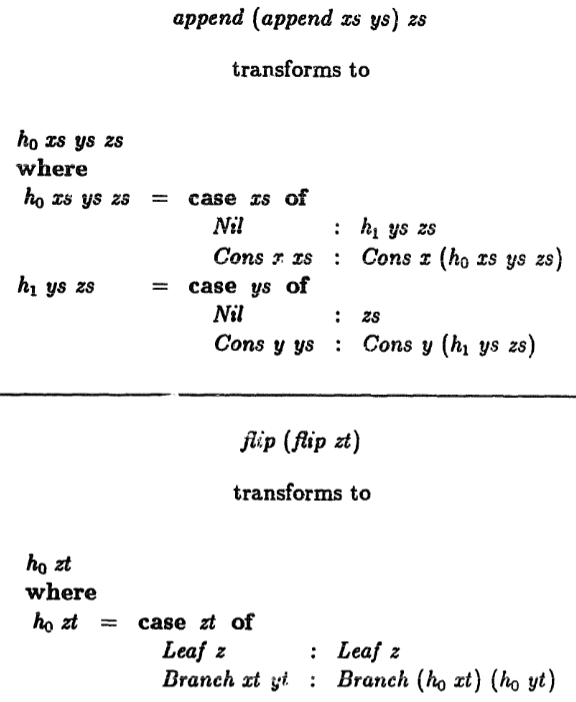
\includegraphics[width=0.6\textwidth]{figs/deforestation-examples}
    \caption{Примеры работы дефорестирующего алгоритма~\cite{wadler1988deforestation}.}
    \label{fig:deforestation-examples}
\end{figure}

Сфокусируемся на списках и рассмотрим более практичные решения\footnote{\url{https://markkarpov.com/tutorial/ghc-optimization-and-fusion.html}}.
Первым очевидным решением было бы для каждой пары функций, работающих со списками, добавить специальное правило переписывания (см.~\ref{subsubsec:rules}), дефорестирующее с помощью алгебраических свойств списочных трансформаций.
Однако, таких правил будет экспоненциально много.
\begin{minted}{haskell}
    {-# RULES
    "map/map" forall f g xs. map f (map g xs) = map (f . g) xs
      #-}
\end{minted}

Современная техника дефорестирования в Haskell --- fold/build list fusion~\cite{gill1993short} --- вместо использования множества алгебраических правил, определяет универсальный способ конструирования и деконструирования списка.
Деконструировать список будем с помощью \mintinline{haskell}|foldr|.
Конструировать будем с помощью функции \mintinline{haskell}|build|:
\begin{minted}{haskell}
    build :: (forall b . (a -> b -> b) -> b -> b) -> [a]
    build g = g (:) []
\end{minted}
Например, список \mintinline{haskell}{[1, 2, 3]} и функция \mintinline{haskell}{map} теперь запишутся следующим образом\footnote{В стандартной библиотеке Haskell функции работы со списками написаны нормально, но рядом написаны правила \texttt{RULES} (см.~\ref{subsubsec:rules}), которые подменяют их реализацию на fold/build.}:
\begin{minted}{haskell}
    list123 :: [Int]
    list123 = build \s z -> s 1 (s 2 (s 3 z))

    map :: (a -> b) -> [a] -> [b]
    map f xs = build \s z -> foldr (\x acc -> s (f x) acc) z xs
\end{minted}
Можно заметить, что на вход \texttt{build} передаётся список Чёрча, отсюда не удивителен закон:
\begin{minted}{haskell}
    foldr f ini (build g) ?$\equiv$? g f ini
\end{minted}

Таким образом, мы избавились от конструирования списков путём замены вызовов конструкторов на вызовы сворачивающих функций.

Дефорестацию также можно производить вручную (см.~\ref{fig:cpp-deforestation}).
\begin{figure}
    \centering
    \begin{tabular}{p{0.5\textwidth} rl}
        \begin{minipage}[t]{0.5\textwidth}
            \begin{minted}{cpp}
                std::variant<Msg1, Msg2>
                    deserialize(bytes bs) {
                    if (...) {
                        return std::variant{Msg1(...)};
                    else {
                        return std::variant{Msg2(...)};
                    }
                }
            \end{minted}
        \end{minipage}
        &
        \begin{minipage}[t]{0.5\textwidth}
            \begin{minted}{cpp}
                template<class Impl>
                auto deserialize(bytes bs) {
                    if (...) {
                        return Impl::processMsg1(...);
                    else {
                        return Impl::processMsg2(...);
                    }
                }
            \end{minted}
        \end{minipage}
    \end{tabular}
    \caption{Ручная дефорестация в C++.}
    \label{fig:cpp-deforestation}
\end{figure}

\subsubsection{Visitor pattern} \label{subsubsec:visitor}

Рассмотрим некоторое дерево и его свёртку:
\begin{minted}{haskell}
    data Tree a = Leaf | Node a [Tree a]
    foldTree :: Tree a -> r -> (a -> [r] -> r) -> r
\end{minted}

Перепишем и переименуем:
\begin{minted}{haskell}
    data Visitor a r = Visitor { onLeaf :: r, onNode :: a -> [r] -> r }
    visitTree :: Tree a -> Visitor a r -> r
\end{minted}

Чтобы это ещё более выглядело в ООП стиле, само дерево должно задаваться свёрткой (как бы интерфейсом с функцией \texttt{visit}), а разные вершины --- конкретными её реализациями (объектами-наследниками):
\begin{minted}{haskell}
    data Tree a = Tree { visit :: forall r . Visitor a r -> r }

    leaf :: Tree a
    leaf = Tree { visit = \Visitor{onLeaf} -> onLeaf }

    node :: a -> [Tree a] -> Tree a
    node x ts = Tree { visit = \v@Visitor{onNode} -> onNode x (map (`visit` v) ts) }
\end{minted}

Для наглядности, покажем этот код ещё и на Kotlin:
\begin{minted}{kotlin}
    interface Visitor<a, r> {
        fun onLeaf(): r
        fun onNode(x: a, subtrees: List<r>): r
    }

    interface Tree<a> {
        fun <r> visit(visitor: Visitor<a, r>): r
    }
    class Leaf : Tree<Nothing> {
        override fun <r> visit(visitor: Visitor<Nothing, r>): r = visitor.onLeaf()
    }
    class Node<a>(val value: a, val subtrees: List<Tree<a>>) : Tree<a> {
        override fun <r> visit(visitor: Visitor<a, r>): r =
            visitor.onNode(value, subtrees.map { it -> it.visit(visitor) })
    }
\end{minted}

\subsection{Всё через развёртку} \label{subsec:all-unfolds}

Вспомним, что существует универсальная развёртка --- анаморфизм, которая по генерирующей процедуре позволяет получить целую структуру данных (см.~\ref{subsubsec:recursion-schemas}).
\begin{minted}{haskell}
    ana :: Functor f => forall s . (s -> f s) -> s -> Fix f
    ana psi = In . fmap (ana psi) . psi
\end{minted}

Приведём функцию \texttt{ana} к типу вида \mintinline{haskell}{A -> B}, чтобы затем проще было исследовать стрелку \mintinline{haskell}{B -> A}.
Для этого сделаем \texttt{uncurry} и перенесём квантор налево от стрелки (он изменится на противоположный):
\begin{minted}{haskell}
    ana :: Functor f => (exists s . (s, s -> f s)) -> Fix f
\end{minted}
Закодируем квантор существования с помощью нового типа (см.~\ref{subsubsec:existentials}) и перепишем анаморфизм на работу с ним:
\begin{minted}{haskell}
    data Box f where
      --     exists s. (s,    s -> f s)
      Box :: forall s . s -> (s -> f s) -> Box

    ana' :: Functor f => Box f -> Fix f
    ana' (Box currSeed psi) =
      In $ (\nextSeed -> ana' (Box nextSeed psi)) <$> psi currSeed
\end{minted}
Теперь построим изоморфизм между структурами данных и их тривиальными развёртками, возвращающими каждый раз следующий слой данной структуры, \mintinline{haskell}|Fix f ?$\simeq$? Box f|:
\begin{minted}{haskell}
    to :: Fix f -> Box f
    to x = Box x out

    from :: Functor f => Box f -> Fix f
    from = ana'
\end{minted}
Таким образом, мы получили свидетельство того, что любую рекурсивную структуру данных можно хотя бы тривиальным образом представить как \mintinline{haskell}{Box f}.
Иногда такое представление называют \vocab{co-Church encoding}~\cite{gibbons2008unfolding}.

Например, бесконечный ленивый список натуральных чисел может быть задан следующим образом.
Заметьте, что тут мы \point{не полагаемся на ленивость Haskell}, а значит можем использовать эту технику и в энергичных языках.
\begin{minted}{haskell}
    nats :: Box (ListF Int)
    nats = Box 0 \curr -> Cons curr (curr + 1)
\end{minted}

\begin{task}
    Реализуйте ленивую функцию \\ \mintinline{haskell}{take :: Int -> Box (ListF Int) -> Box (ListF Int)}.
\end{task}

Иначе говоря, бесконечные структуры данных представимы как процедуры, лениво генерирующие слой рекурсивной структуры за слоем по запросу.

\subsubsection{Абстрактные типы данных} \label{subsubsec:abstract-data-types}

Рассмотрим случай, когда функтор формы представляет собой произведение:
\[
    \text{\texttt{s -> f s}} \iso \left( \prod_{i}(t_i\ap s) \right)^{\displaystyle s} \iso \prod_i(s\to t_i\ap s)
\]
То есть коалгебра эквивалентна кортежу функций.
Таким образом, \mintinline{haskell}{Box} это не что иное, как \point{абстрактный тип данных (ADT)}: он включает в себя скрытое состояние неизвестной природы и набор операций для работы с ним~\cite{gibbons2008unfolding}.
На самом деле мы уже встречали такую конструкцию ранее, когда говорили про экзистенциальные типы~\ref{subsubsec:existentials} (там мы использовали инстансы классы типов в качестве кортежей функций).

Известно, что ООП объекты тоже имеют коалгебраическую природу.
Подробнее про соотношение объектов и абстрактных типов данных можно почитать в~\cite{cook2009understanding}.

% todo Pierce about data abstraction

\subsubsection{Stream fusion} \label{subsubsec:stream-fusion}

Ранее мы рассматривали foldr/build list fusion оптимизацию, элиминирующую промежуточные списки (см.~\ref{subsubsec:deforestation-fusion}).
Однако, эта техника не подходит для многих популярных функций, например, \texttt{zip} (нужно корутинить между двумя алгебрами) или \texttt{take} (нужно оборвать свёртку в определённый момент).

Позднее была предложена техника использования ко-структуры списка --- развёртки или \mintinline{haskell}{Stream}\footnote{\url{https://markkarpov.com/tutorial/ghc-optimization-and-fusion.html}}~\cite{coutts2007stream}:
\begin{minted}{haskell}
    data ListF a r = Nil | Cons a r
    type MyStream a = Box (ListF a) -- ?$\exists$?s . (s -> ListF a s, s)
    -- ?$\iso$?
    data Step a s = Done | Yield a s
    data Stream a where
      Stream :: forall s . (s -> Step a s) -> s -> Stream a

    stream :: [a] -> Stream a
    stream xs = Stream (\case [] -> Done; x:xs -> Yield x xs) xs

    unstream :: Stream a -> [a]
    unstream (Stream next s) = case next s of
      Done -> []
      Cons a s' -> a : unstream next s'
\end{minted}

Идея в том, что теперь \point{функции работы со стримами нерекурсивны} и легко подвергаются базовым компиляторным дефорестирующим трансформациям в стиле~\cite{wadler1988deforestation}.
Действительно, вместо рекурсивного вызова мы запоминаем состояние для следующей итерации.
\begin{minted}{haskell}
    mapS :: (a -> b) -> Stream a -> Stream b
    mapS f (Stream next s) = Stream next' s
      where
        next' s = case next s of
          Done -> Done
          Yield x s' -> Yield (f x) s'
\end{minted}

Общий пайплайн выглядит следующим образом:
\begin{enumerate}
    \item Мы пишем все функции работы со списками через стримы:
    \begin{minted}{haskell}
        map :: (a -> b) -> [a] -> [b]
        map f = unstream . map f . stream
    \end{minted}
    \item С помощью RULES (см.~\ref{subsubsec:rules}) задаём правило переписывания stream/unstream, двойственное foldr/build: \texttt{stream . unstream = id}.
    \item Далее справляются обычные компиляторные оптимизации.\footnote{Можно гарантировать полную дефорестацию с помощью staging (см. далее~\ref{sec:datatype-generic})~\cite{kiselyov2017stream}.}
\end{enumerate}

Чтобы поддержать нерекурсивную функцию фильтрации, обычно добавляют отдельный вид шагов:
\begin{minted}{haskell}
    data Step a s = Done | Skip s | Yield a s

    filterS :: (a -> Bool) -> Stream a -> Stream a
    filterS p (Stream next s) = Stream next' s
      where
        next' s = case next s of
          Done -> Done
          Skip s' -> Skip s'
          Yield a s' -> if p a then Yield a s' else Skip s'
\end{minted}

В стандартной библиотеке Haskell всё-таки используется foldr/build fusion, однако существует множество промышленных библиотек стримов~\cite[глава 14]{bragilevsky-haskell}.

Больше про стримы можно почитать у Олега Киселёва\footnote{\url{https://okmij.org/ftp/Streams.html}}.

\subsection{Вездесущий дуализм} \label{subsec:data-duality}

Мы рассмотрели три формы рекурсивных данных:
\begin{itemize}
    \item \mintinline{haskell}{Fix f} --- обычные рекурсивные типы данных, конечные в энергичных языках;
    \item \mintinline{haskell}{?$\forall$?a . (f a -> a) -> a} --- Church encoding, конечные структуры заданные свёртками;
    \item \mintinline{haskell}{?$\exists$?s . (s -> f s, s)} --- co-Church encoding, потенциально бесконечные структуры данных, абстракции по данным (работаем через интерфейс над сокрытым представлением).
\end{itemize}

В этом разделе мы рассмотрим некоторые практические примеры, в которых пространство решений задано дуальными представлениями коллекций.

\subsubsection{Push vs pull streaming} \label{subsubsec:push-pull}

Рассмотрим различные представления списков или, как их иногда называют, потоков событий.
Подробнее сравнение можно посмотреть тут~\cite[параграф 3]{kiselyov2017stream}.

Church encoding для списков даёт \vocab{push stream}, или \vocab{internal iteration}, или \vocab{Observer pattern}\footnote{\url{https://learn.microsoft.com/en-us/dotnet/api/system.iobserver-1?view=net-9.0}} (в некотором смысле частный случай Visitor pattern~\ref{subsubsec:visitor}), когда мы регистрируем обработчика событий, а коллекция вызывает (push) на нём методы.
Примерами push потоков являются Java Stream API\footnote{\url{https://docs.oracle.com/javase/8/docs/api/java/util/stream/Stream.html}}, Closure Transducers\footnote{\url{https://clojure.org/reference/transducers}}.
\begin{minted}{kotlin}
    events.observe(object : Observer<Event> {
        override fun onComplete() { .. }
        override fun onNext(elem: Event) { .. }
    })
\end{minted}

co-Church encoding для списков даёт \vocab{pull stream}, или \vocab{external iteration}, или \vocab{Iterator pattern}.
Чтобы получить следующий элемент, его нужно явно запросить (pull) потребляющему коду.
Это представление часто гораздо удобнее с точки зрения использования (см.~\ref{subsubsec:stream-fusion})\footnote{\url{https://github.com/pulldown-cmark/pulldown-cmark/?tab=readme-ov-file\#why-a-pull-parser}}, однако сложнее на стороне имплементации, потому что нужно выделить и поддерживать экзистенциальное состояние в коалгебре.
Генераторы призваны автоматизировать выделение этого состояния, так как можно заметить, что это continuation вычисления (см. далее~\ref{sec:continuations}).

Нередко работу с потоками называют \vocab{реактивным программированием}\footnote{\href{https://youtu.be/sTSQlYX5DU0?si=Xhfi62ScXHBBjdBx}{(youtube) React 2014 : Erik Meijer - What does it mean to be Reactive?}}.
Чистой версией является \vocab{functional reactive programming (FRP)}, представляющее потоки как функции от времени\footnote{\href{https://youtu.be/rfmkzp76M4M?si=TRBq8wWbcDOhSbIO}{(youtube) Conal Elliott - The Essence \& Origins of Functional Reactive Programming}}~\cite{elliott1997functional}.

\subsubsection{Data vs codata} \label{subsubsec:data-codata}

Вспомним функтор-формы для списка:
\begin{minted}{haskell}
    data ListF a r = Nil | Cons a r
\end{minted}

С помощью ключевого слова \mintinline{haskell}{data} мы определяем новый алгебраический тип данных через способы его сконструировать.
Далее, с помощью pattern-matching мы можем деконструировать значения алгебраического типа данных и воспользоваться хранящейся в нём информацией.
\begin{minted}{haskell}
    data List a where
      List :: ListF a (List a) -> List a

    fold :: (ListF a r -> r) -> List a -> r
    fold alg xs = case xs of
      Fix Nil -> alg Nil
      Fix (Cons y ys) -> alg (Cons y (fold alg ys))
\end{minted}

Однако, также можно определять тип данных через способы его деконструировать с помощью ключевого слова \mintinline{haskell}{codata} (в воображаемом языке).
Так, у ко-списка можно потребовать показать следующий слой структуры.
Сконструировать такой тип данных можно с помощью co-pattern-matching'а, описав как деконструирующая функция должна вести себя на конструирующем терме (\texttt{unfold coalg s})\footnote{\href{https://youtu.be/ZCdYIEwcna0?si=XEQSBFhnehQFZPxy}{(youtube) CS410 2017 Lecture 15 Coinduction and Coalgebras}}.
\begin{minted}{haskell}
    codata CoList a where
      force :: CoList a -> ListF a (CoList a)

    unfold :: (s -> ListF a s) -> s -> CoList a
    force (unfold coalg s) = case coalg s of
      Nil -> Nil
      Cons x s' -> Cons x (unfold coalg s')
\end{minted}

По сути, \mintinline{haskell}{codata} представляет собой словарь функций, которые захватывают некоторое состояние, необходимое для генерации следующих слоёв структуры.
Так, \mintinline{haskell}{codata} можно сравнить с ООП интерфейсами, а co-pattern-matching с анонимной реализацией интерфейса.
Предыдущие два примера можно записать, например, в Kotlin следующим образом (форма списка кодируется как \mintinline[escapeinside=**]{kotlin}|Pair<a, r>?|, убедитесь самостоятельно, что этот тип изоморфен \mintinline{haskell}{ListF}).
\begin{minted}[escapeinside=**]{kotlin}
    class List<a>(val layer: Pair<a, List<a>>?)

    fun <a, r> fold(alg: (Pair<a, r>?) -> r, xs: List<a>): r =
        if (xs.layer == null) alg(null)
        else alg(Pair(xs.layer.first, fold(alg, xs.list.second)))

    interface CoList<a> { fun force(): Pair<a, CoList<a>>? }

    fun <a, s> unfold(coalg: (s) -> Pair<a, s>?, ini: s): CoList<a> =
        object : CoList<a> {
            override fun force(): Pair<a, CoList<a>>? {
                val layer = coalg(ini)
                return if (layer == null) null else
                    Pair(layer.first, unfold(coalg, layer.second))
            }
        }
\end{minted}

Функциональный стиль программирование в основном оперирует напрямую наблюдаемыми данными \mintinline{haskell}{data}, а ООП --- скрывает данные за интерфейсами \mintinline{haskell}{codata}.
Однако, обе конструкции имеют свои понятные области применения и ими не стоит пренебрегать вне зависимости от предпочитаемого стиля~\cite{downen2019codata}\footnote{\url{https://reasonablypolymorphic.com/blog/review-codata/}}.

В языках с проверкой тотальности функций разделяют индуктивные и коиндуктивные определения.
Для них используются паттерн-матчинг и ко-паттерн-матчинг, принцип индукции (катаморфизм) и принцип коиндукции (анаморфизм).
Индуктивные определения задают конечные структуры данных, проверка тотальности проверяет, что рекурсивные вызовы делаются на структурно меньших подтермах.
Коиндуктивные определения задают потенициально бесконечные структуры данных, для них проверяется продуктивность --- порождающая функция всегда после рекурсивного вызова породит новый конструктор~\footnote{\url{https://rocq-prover.org/doc/V8.18.0/refman/language/core/coinductive.html}}.

% todo \vocab{полярности}\footnote{\url{https://existentialtype.wordpress.com/2012/08/25/polarity-in-type-theory/}}\footnote{\url{https://ncatlab.org/nlab/show/polarity+in+type+theory}}

\subsection{Приложение: категория алгебр} \label{subsec:cats}

Это факультативный раздел, не являющийся необходимым для понимания курса в дальнейшем.
Однако, полезен для понимания часто употребимой терминологии.

\vocab{Категория} --- это коллекция объектов и коллекция стрелок.
Для каждого объекта $X$ существует тождественная стрелка, а для каждой пары стрелок существует способ получить их композицию: $f : Y \to Z, g : X \to Y \Rightarrow f \circ g : X \to Z$.

Определяют категорию, соответствующую Haskell --- $Hask$.
На самом деле это плохая категория с точки зрения теории, но для наших нестрогих рассуждений подойдёт\footnote{\url{https://math.andrej.com/2016/08/06/hask-is-not-a-category/}}.
Объектами в Hask являются типы языка Haskell, а морфизмами --- термы, задающие функции между соответствующими типами.
Тождественный морфизм --- \mintinline{haskell}|id|, композиция задаётся как \mintinline{haskell}|f . g = \x -> f (g x)|.

\begin{task}
    Как в такой категории представить константы?
\end{task}

\vocab{Функтором} называется отображение между категориями, которое объектам одной категории сопоставляет объекты другой, а стрелкам одной --- стрелки другой.
В Haskell типовые конструкторы задают отображение между объектами, а \mintinline{haskell}|fmap| --- между стрелками.
Функтор должен сохранять тождественный морфизм и композицию.
\begin{figure}[h!]
    \centering
    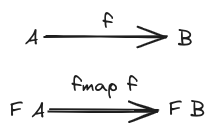
\includegraphics[width=0.25\textwidth]{figs/functor}
\end{figure}

\vocab{Алгеброй} в категории $C$ называется пара из объекта категории $X \in Obj(C)$ и морфизма $\phi : F\ap X \to X$, где $F$ --- функтор.
Сам морфизм $F\ap X \to X$ называют \vocab{f-алгеброй}.
Алгебрами в смысле категорий можно описывать алгебры.
Так, в качестве объекта $X$ берём носитель алгебры.
В качестве функтора $F$ --- сигнатуру алгебры в виде типа-формы.
Тогда морфизмом будет интерпретацией сигнатуры.

\vocab{Морфизмом алгебр} называется такой морфизм между носителями $h : X \to Y$, что следующая диаграмма коммутирует.
Говорят, что \vocab{диаграмма коммутирует}, если все возможные пути по стрелкам в ней равны.
\begin{figure}[h!]
    \centering
    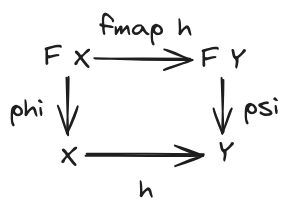
\includegraphics[width=0.3\textwidth]{figs/alg-homomorphism}
\end{figure}

В морфизме алгебр можно обнаружить знакомые черты гомоморфизмов, то есть операций между носителями, которые ``уважают'' операции сигнатуры алгебраической теории.

Алгебры над категорией $C$ образуют \vocab{категорию алгебр}, в которой объектами являются алгебры, а морфизмами --- морфизмы алгебр.

\vocab{Начальным (инициальным) объектом} категории называется объект, из которого в каждый другой объект существует уникальная стрелка.
\vocab{Терминальным (финальным) объектом} категории называется объект, в который из каждого другого объекта категории существует уникальная стрелка.

Инициальный и терминальный объекты категории не обязательно присутствуют в единственном экземпляре.
Но все инициальные объекты изоморфны друг другу, как и все терминальные.

\begin{task}
    Приведите начальный и терминальный объекты категории $Hask$.
\end{task}

Рекурсивный тип --- это тип, значит ему соответствует объект в категории Hask.
$X$ является рекурсивным типом с формой $F$, если имеет место следующий изоморфизм:
\[X \simeq F\ap X\]

Можно заметить, что свидетель изоморфизма справа налево напоминает f-алгебру, а слева направо --- f-коалгебру (всё то же самое, только все стрелки в обратную сторону).
И действительно, подходящий объект $X$ должен быть либо начальным объектом категории алгебр, либо терминальным объектом категории коалгебр (с соответствующими морфизмами).
Первый вариант соответствует конечным структурам данных, второй --- потенциально бесконечным.

Начальным объектом категории алгебр над $Hask$ для функтора $f$ является следующая алгебра: \mintinline{haskell}|(Fix f, In)|\footnote{\url{https://bartoszmilewski.com/2017/02/28/f-algebras/}}\footnote{\url{https://ncatlab.org/nlab/show/catamorphism}}. % todo проверить инициальность свёрток
Действительно, для каждого типа \texttt{a} и для каждой f-алгебры \texttt{phi} мы можем построить такой морфизм \mintinline{haskell}|cata phi :: Fix f -> a|, что следующая диаграмма будет коммутировать:
\begin{figure}[h!]
    \centering
    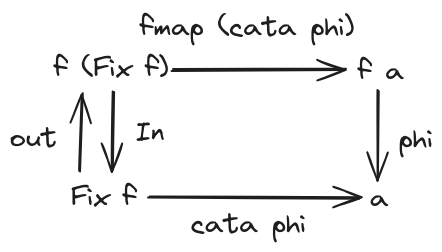
\includegraphics[width=0.4\textwidth]{figs/cata}
\end{figure}

Покажем, что \mintinline{haskell}|(Fix f, out)| является терминальным объектом категории коалгебр (благодаря ленивости Haskell). % todo как тут учитывается ленивость % todo проверить калгебраические стреллки
Аналогично, для каждого объекта \texttt{a} и f-коалгебры \texttt{psi} найдётся морфизм \mintinline{haskell}|ana psi :: a -> Fix f|:
\begin{figure}[h!]
    \centering
    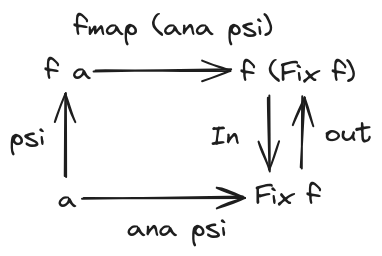
\includegraphics[width=0.35\textwidth]{figs/ana}
\end{figure}

% todo про пределы и копределы
